% =====================================================================
% Trabalho de VE - Mecânica II - CFG 2026 - Grupo I (Pião)
% Compilação: pdflatex relatorio_grupo_I.tex  (executar 3 vezes, para que
% sumário, lista de figuras e referências cruzadas fiquem atualizados).
% As figuras são geradas por scripts/calculos_e_graficos.py
% =====================================================================
\documentclass[12pt,a4paper]{article}

\usepackage[utf8]{inputenc}
\usepackage[T1]{fontenc}
\usepackage{lmodern}
\usepackage[brazil]{babel}
\usepackage[a4paper,top=3cm,bottom=2.5cm,left=3cm,right=2.5cm]{geometry}
\usepackage{amsmath,amssymb}
\usepackage{icomma}
\usepackage{graphicx}
\usepackage{tikz}
\usetikzlibrary{arrows.meta,calc}
\definecolor{azul}{HTML}{2A78D6}
\definecolor{laranja}{HTML}{EB6834}
\definecolor{tinta2}{HTML}{52514E}
\definecolor{apoio}{HTML}{E3E1DA}
\definecolor{corpo}{HTML}{F4E6DC}
\definecolor{corpoesc}{HTML}{DDBBA6}
\definecolor{corpob}{HTML}{A9765A}
\usepackage{float}
\usepackage[titles]{tocloft}
\renewcommand{\cftfigpresnum}{Figura~}
\renewcommand{\cftfigaftersnum}{ --}
\setlength{\cftfignumwidth}{5.8em}
\setlength{\cftfigindent}{0pt}
\setlength{\cftbeforefigskip}{4pt}
\usepackage{booktabs}
\usepackage{array}
\usepackage{setspace}
\usepackage{indentfirst}
\usepackage[font=small,labelfont=bf,labelsep=endash]{caption}
\usepackage[hidelinks]{hyperref}

\graphicspath{{figuras/}}
\onehalfspacing
% mesmo espaçamento vertical em torno de todas as equações
\makeatletter
\g@addto@macro\normalsize{%
  \setlength\abovedisplayshortskip{\abovedisplayskip}%
  \setlength\belowdisplayshortskip{\belowdisplayskip}}
\makeatother

% Notação: vetores e tensores em negrito; magnitudes em itálico (padrão do modo matemático)
\newcommand{\vet}[1]{\mathbf{#1}}
\newcommand{\vomega}{\boldsymbol{\omega}}
\newcommand{\vOmega}{\boldsymbol{\Omega}}
\newcommand{\seno}{\operatorname{sen}}
\newcommand{\un}[1]{\,\mathrm{#1}}
\newcommand{\phid}{\dot{\phi}}
\newcommand{\psid}{\dot{\psi}}
\newcommand{\eps}{\varepsilon}

\begin{document}
\pagenumbering{roman}

% ------------------------------------------------------------- capa
\begin{center}
\thispagestyle{empty}
{\large\textbf{INSTITUTO MILITAR DE ENGENHARIA}}\\[0.3cm]
{Curso de Formação e Graduação (CFG) -- 2.\textsuperscript{o} ano -- Turma A}\\[0.1cm]
{Mecânica II -- Dinâmica de Corpos Rígidos}

\vspace{3cm}

{\LARGE\textbf{PIÃO: PRECESSÃO PERMANENTE}}\\[0.5cm]
{\large Trabalho de VE -- Grupo I}

\vspace{2.5cm}

\begin{tabular}{l}
\textbf{Componentes:}\\[0.15cm]
João Eduardo Moro Hoffmann\\
Maria Eduarda Medina Henriques\\
Gabriela de Lima Cardoso\\
Sara Eduarda dos Santos Borges\\
Lucas Santos Moraes\\
Cláudio Erick de Holanda Fontenele\\
Tiago Alves Porto Lima\\
Marcos Kalile Meira de Vasconcellos
\end{tabular}

\vfill
Rio de Janeiro\\
Novembro de 2026
\end{center}
\clearpage

% ------------------------------------------------------------- listas
\tableofcontents
\clearpage

\phantomsection
\addcontentsline{toc}{section}{Lista de Figuras}
\listoffigures
\clearpage

\phantomsection
\addcontentsline{toc}{section}{Lista de Símbolos}
\section*{Lista de Símbolos}

{\small
\setstretch{1.0}
\renewcommand{\arraystretch}{1.1}
\noindent
\begin{tabular}{@{}l p{9.3cm} l@{}}
\toprule
\textbf{Símbolo} & \textbf{Significado} & \textbf{Unidade}\\
\midrule
$a$ & coeficiente $(I'-I)\cos\theta$ da equação de segundo grau & kg$\cdot$m$^2$\\
$b$ & coeficiente $I\psid$ da equação de segundo grau & kg$\cdot$m$^2$/s\\
$c$ & distância do ponto $O$ ao centro de gravidade $G$ & m\\
$E$ & energia mecânica total do pião & J\\
$e$ & erro relativo da aproximação de alta rotação & \%\\
$g$ & aceleração da gravidade & m/s$^2$\\
$\vet{H}_O$ & quantidade de movimento angular em relação a $O$ & kg$\cdot$m$^2$/s\\
$\vet{I}_O$ & tensor de inércia em relação a $O$ & kg$\cdot$m$^2$\\
$I$ & momento de inércia em relação ao eixo de simetria & kg$\cdot$m$^2$\\
$I'$ & momento de inércia em relação a um eixo transversal por $O$ & kg$\cdot$m$^2$\\
$\vet{i},\ \vet{j},\ \vet{k}$ & vetores unitários dos eixos $x$, $y$ e $z$ & --\\
$\vet{K}$ & vetor unitário do eixo vertical fixo $Z$ & --\\
$k$ & raio de giração em relação ao eixo de simetria & m\\
$k'$ & raio de giração em relação ao eixo transversal por $O$ & m\\
$L$ & função lagrangiana do pião & J\\
$\vet{M}_O$ & momento resultante em relação a $O$ & N$\cdot$m\\
$m$ & massa do pião & kg\\
$\vet{N}$ & componente vertical da reação em $O$ & N\\
$p_\phi,\,p_\psi$ & quantidades de movimento generalizadas conservadas & kg$\cdot$m$^2$/s\\
$\vet{q}$ & quatérnio unitário de orientação do pião & --\\
$\vet{R}_h$ & componente horizontal da reação em $O$ & N\\
$\vet{r}_G$ & vetor posição de $G$ em relação a $O$ & m\\
$t$ & tempo & s\\
$\vet{W}$ & peso do pião & N\\
$\eps$ & parâmetro adimensional $aWc/b^2$ & --\\
$\theta$ & ângulo de nutação (entre os eixos $Z$ e $z$) & rad\\
$\theta_0,\ \phid_0$ & valores iniciais de $\theta$ e $\phid$ nas simulações & rad; rad/s\\
$\phi,\ \phid$ & ângulo e taxa de precessão & rad; rad/s\\
$\phid_1,\ \phid_2$ & taxas de precessão permanente lenta e rápida & rad/s\\
$\phid_a$ & taxa de precessão da aproximação de alta rotação & rad/s\\
$\psi,\ \psid$ & ângulo e taxa de rotação própria (\textit{spin}) & rad; rad/s\\
$\psid_{\mathrm{min}}$ & menor \textit{spin} que admite precessão permanente & rad/s\\
$\vomega$ & velocidade angular do pião & rad/s\\
$\omega_z$ & componente de $\vomega$ segundo o eixo de simetria & rad/s\\
$\omega_{z,\mathrm{min}}$ & menor valor de $\omega_z$ que estabiliza o pião na vertical & rad/s\\
$\vOmega$ & velocidade angular do referencial $Oxyz$ & rad/s\\
\bottomrule
\end{tabular}
}
\clearpage

\pagenumbering{arabic}

% ------------------------------------------------------------- 1
\section{Introdução}

Um pião em repouso, apoiado sobre a própria ponta, tomba imediatamente. Basta, porém, colocá-lo em rotação rápida para que ocorra algo que contraria a intuição: mesmo inclinado, o pião não cai. O seu eixo passa a descrever, lentamente, um cone em torno da vertical, como se a gravidade, em vez de derrubá-lo, o empurrasse para o lado. Esse movimento recebe o nome de precessão.

O brinquedo esconde um princípio de grande alcance tecnológico. O mesmo fenômeno governa os giroscópios e as girobússolas empregados em sistemas de navegação inercial, a estabilização de projéteis por rotação e a orientação de satélites. Em escala astronômica, o eixo de rotação da Terra precessa de modo análogo sob a ação gravitacional do Sol e da Lua. Compreender o pião significa, portanto, compreender a base física desses sistemas.

Este trabalho analisa a precessão permanente de um pião de massa e geometria conhecidas, conforme proposto ao Grupo I. Determinam-se as taxas de precessão possíveis para inclinações entre $30^\circ$ e $60^\circ$, deduz-se a condição simplificada válida para rotação muito rápida e quantifica-se o erro cometido ao utilizá-la. Como aprofundamento, investigam-se a existência das soluções, as reações no apoio e a razão pela qual apenas uma das duas soluções é observada na prática. Os resultados são verificados por uma integração numérica independente das equações do movimento.

% ------------------------------------------------------------- 2
\section{Desenvolvimento}

\subsection{Descrição do problema e hipóteses}

Um pião de massa $m$ é suportado no ponto fixo $O$, como ilustra a Figura~\ref{fig:piao}. A figura mostra o eixo vertical fixo $Z$, o eixo de simetria $z$ do pião, inclinado do ângulo $\theta$ em relação a $Z$, e o centro de gravidade $G$, situado sobre o eixo de simetria, à distância $c$ do apoio.

\begin{figure}[H]
\centering
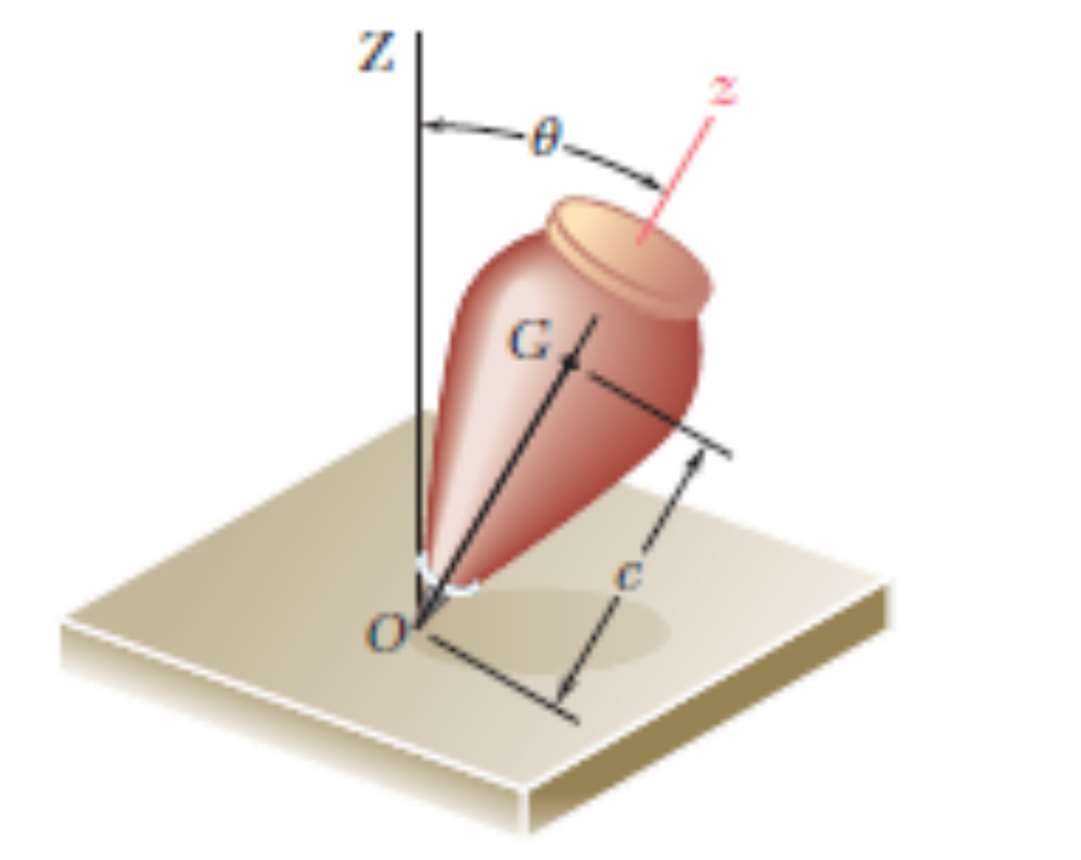
\includegraphics[width=0.35\linewidth]{piao_enunciado.jpg}
\caption[Pião suportado no ponto fixo $O$]{Pião em rotação suportado no ponto fixo $O$, com o eixo de simetria $z$ inclinado de $\theta$ em relação à vertical $Z$ (figura do enunciado do trabalho).}
\label{fig:piao}
\end{figure}

Os dados do problema constam da Tabela~\ref{tab:dados}.

\begin{table}[H]
\centering
\caption{Dados do problema.}
\label{tab:dados}
\begin{tabular}{lcc}
\toprule
\textbf{Grandeza} & \textbf{Símbolo} & \textbf{Valor}\\
\midrule
Massa do pião & $m$ & $100\un{g}=0,100\un{kg}$\\
Raio de giração (eixo de simetria) & $k$ & $25\un{mm}=0,025\un{m}$\\
Raio de giração (eixo transversal por $O$) & $k'$ & $50\un{mm}=0,050\un{m}$\\
Distância de $O$ a $G$ & $c$ & $40\un{mm}=0,040\un{m}$\\
Taxa de rotação própria (\textit{spin}) & $\psid$ & $1800\un{rpm}=188,50\un{rad/s}$\\
Faixa de inclinação & $\theta$ & $30^\circ$ a $60^\circ$\\
\bottomrule
\end{tabular}
\end{table}

Adotam-se as seguintes hipóteses: o pião é um corpo rígido com simetria de revolução em torno do eixo $z$; o ponto $O$ permanece fixo; o atrito é desprezado, de modo que o apoio não exerce momento em relação a $O$ nem há dissipação de energia; a aceleração da gravidade, não fornecida no enunciado, vale $g=9,81\un{m/s^2}$. O sistema de referência adotado é descrito na Figura~\ref{fig:dcl}.

\begin{figure}[H]
\centering
% Figura: referencial Oxyz (a) e diagrama de corpo livre (b).
% theta = 32 graus (esquemático): \S = sen(theta), \C = cos(theta).
\def\S{0.5299}
\def\C{0.8480}
\def\perfilpiao{%
  plot[smooth,tension=0.6] coordinates {(-0.72,3.1) (-1.0,2.85) (-1.05,2.3) (-0.85,1.6)
    (-0.5,0.85) (-0.18,0.25) (0,0) (0.18,0.25) (0.5,0.85) (0.85,1.6) (1.05,2.3) (1.0,2.85) (0.72,3.1)}}%
\begin{tikzpicture}[scale=0.95,baseline=(cap.base),
    x={(0.966cm,0.129cm)},y={(-0.259cm,0.483cm)},z={(0cm,0.866cm)},
    eixo/.style={-{Stealth[length=2.2mm]},tinta2,line width=0.5pt},
    taxa/.style={-{Stealth[length=2mm]},laranja,line width=1pt}]
  % eixo x: abaixo do plano de apoio, portanto desenhado antes dele
  \draw[eixo] (0,0,0) -- ({2.9*\C},0,{-2.9*\S}) node[right,text=black] {$x\ (\mathbf{i})$};
  % plano de apoio translúcido
  \fill[apoio,opacity=0.8] (-2,-2,0) -- (2,-2,0) -- (2,2,0) -- (-2,2,0) -- cycle;
  \draw[tinta2,line width=0.3pt] (-2,-2,0) -- (2,-2,0) -- (2,2,0) -- (-2,2,0) -- cycle;
  % corpo: silhueta alinhada à projeção do eixo z
  \begin{scope}[x=1cm,y=1cm,rotate=-32.6,yscale=0.95]
    \shade[left color=corpoesc,right color=corpoesc,middle color=corpo,draw=corpob,line width=0.5pt]
      \perfilpiao -- cycle;
    \draw[fill=corpo,draw=corpob,line width=0.5pt] (0,3.1) ellipse (0.72 and 0.22);
  \end{scope}
  % eixos
  \draw[eixo] (0,0,0) -- (0,0,4.8) node[above left,text=black,inner sep=1pt] {$Z\ (\mathbf{K})$};
  \draw[eixo] (0,0,0) -- ({4.9*\S},0,{4.9*\C}) node[right,text=black] {$z\ (\mathbf{k})$};
  \draw[eixo] (0,0,0) -- (0,2.2,0) node[left,text=black,inner sep=1.5pt] {$y\ (\mathbf{j})$};
  % theta, no plano Zz
  \draw[line width=0.5pt] plot[domain=0:32,samples=20] ({1.5*sin(\x)},0,{1.5*cos(\x)});
  \node[inner sep=1pt] at ({1.85*sin(16)},0,{1.85*cos(16)}) {$\theta$};
  % trajetória de G, com o sentido do movimento
  \draw[azul,densely dashed,line width=0.6pt] plot[domain=0:360,samples=90]
    ({2.4*\S*cos(\x)},{2.4*\S*sin(\x)},{2.4*\C});
  \draw[-{Stealth[length=2mm]},azul,line width=0.8pt] plot[domain=20:50,samples=12]
    ({2.4*\S*cos(\x)},{2.4*\S*sin(\x)},{2.4*\C});
  \fill ({2.4*\S},0,{2.4*\C}) circle (1.5pt) node[below right,inner sep=2pt] {$G$};
  \fill (0,0,0) circle (1.5pt) node[below left,inner sep=2pt] {$O$};
  % taxas no sentido positivo (anti-horário visto da ponta de cada eixo)
  \draw[taxa] plot[domain=200:490,samples=50] ({0.42*cos(\x)},{0.42*sin(\x)},4.15);
  \node[left=6pt] at (0,0,4.15) {$\dot{\phi}$};
  \draw[taxa] plot[domain=200:490,samples=50]
    ({4.25*\S+0.42*cos(\x)*\C},{0.42*sin(\x)},{4.25*\C-0.42*cos(\x)*\S});
  \node[right=7pt] at ({4.25*\S},0,{4.25*\C}) {$\dot{\psi}$};
  \node[anchor=north] (cap) at (canvas cs:x=0.35cm,y=-1.45cm) {\small (a) Referencial e movimento};
\end{tikzpicture}\hfill
\begin{tikzpicture}[scale=0.95,baseline=(cap.base),
    eixo/.style={-{Stealth[length=2.2mm]},tinta2,line width=0.5pt},
    forca/.style={-{Stealth[length=2.6mm]},line width=1.3pt}]
  % corpo em vista lateral
  \begin{scope}[rotate=-32]
    \shade[left color=corpoesc,right color=corpoesc,middle color=corpo,draw=corpob,line width=0.5pt]
      \perfilpiao -- cycle;
    \draw[corpob,line width=0.5pt] (-0.72,3.1) -- (0.72,3.1);
  \end{scope}
  % eixos
  \draw[eixo] (0,0) -- (0,4.7) node[above,text=black] {$Z$};
  \draw[eixo] (0,0) -- ({4.9*\S},{4.9*\C}) node[right,text=black] {$z$};
  \draw[eixo] (0,0) -- ({2.1*\C},{-2.1*\S}) node[right,text=black] {$x$};
  % theta
  \draw[line width=0.5pt] (0,1.65) arc[start angle=90,end angle=58,radius=1.65];
  \node[inner sep=1pt] at (0.51,1.92) {$\theta$};
  % cota c, paralela ao eixo z
  \coordinate (A) at ({-1.55*\C},{1.55*\S});
  \coordinate (B) at ({-1.55*\C+2.4*\S},{1.55*\S+2.4*\C});
  \draw[tinta2,densely dotted,line width=0.4pt] (0,0) -- (A);
  \draw[tinta2,densely dotted,line width=0.4pt] ({2.4*\S},{2.4*\C}) -- (B);
  \draw[{Stealth[length=1.8mm]}-{Stealth[length=1.8mm]},line width=0.4pt] (A) -- (B)
    node[midway,above left,inner sep=1pt] {$c$};
  % forças
  \draw[forca,laranja] ({2.4*\S},{2.4*\C}) -- ++(0,-1.6) node[right,text=black,inner sep=2pt] {$\mathbf{W}$};
  \draw[forca,azul] (0,0) -- (0,1.05) node[left,text=black,inner sep=2pt] {$\mathbf{N}$};
  \draw[forca,azul] (0,0) -- (-1.05,0) node[below,text=black,inner sep=2pt] {$\mathbf{R}_h$};
  \fill ({2.4*\S},{2.4*\C}) circle (1.5pt) node[above right,inner sep=2pt] {$G$};
  % O com o eixo y entrando no plano (símbolo: círculo com X)
  \draw[fill=white,line width=0.5pt] (0,0) circle (2.6pt);
  \draw[line width=0.5pt] (-1.84pt,-1.84pt) -- (1.84pt,1.84pt) (-1.84pt,1.84pt) -- (1.84pt,-1.84pt);
  \node[below,inner sep=4pt] at (0,0) {$O$};
  \node[anchor=north,align=center,font=\footnotesize] at (-0.35,-0.62) {$y$ entra no plano};
  \node[anchor=north] (cap) at (0.45,-1.45) {\small (b) Diagrama de corpo livre};
\end{tikzpicture}

\caption[Referencial $Oxyz$ e diagrama de corpo livre do pião]{Referencial $Oxyz$ e forças no pião: (a) vista em perspectiva, com os eixos, as taxas $\dot{\phi}$ e $\dot{\psi}$ no sentido positivo e a trajetória de $G$ (linha tracejada); (b) diagrama de corpo livre no plano $Zz$, com o peso $\vet{W}$ em $G$ e as reações $\vet{N}$ e $\vet{R}_h$ em $O$. Representação esquemática, sem escala.}
\label{fig:dcl}
\end{figure}

Na Figura~\ref{fig:dcl}(a), o eixo $z$ coincide com o eixo de simetria, o eixo $x$ pertence ao plano vertical que contém $Z$ e $z$, e o eixo $y$ é perpendicular a esse plano, formando um triedro direto. Adota-se a convenção do livro-texto, na qual $\vet{K}\cdot\vet{i}=-\seno\theta$: por essa razão, o eixo $x$ aponta para baixo do plano horizontal, e o eixo $y$, dado por $\vet{j}=\vet{k}\times\vet{i}$, entra no plano da Figura~\ref{fig:dcl}(b). Trata-se de eixos geométricos de referência, e não de partes do pião. A linha tracejada indica a circunferência horizontal descrita por $G$. O referencial $Oxyz$ acompanha a precessão, mas não a rotação própria do pião. Como o pião é simétrico em torno de $z$, os eixos $Oxyz$ permanecem eixos principais de inércia, ainda que não sejam solidários ao corpo. As únicas forças externas são o peso e a reação no apoio; esta última não produz momento em relação a $O$, razão pela qual o ponto $O$ é escolhido como referência.

\subsection{Cinemática e propriedades de inércia}

Segue-se a formulação de Beer, Johnston e Cornwell \cite{beer}. A orientação do pião é descrita pelos ângulos de Euler: precessão $\phi$, nutação $\theta$ e rotação própria $\psi$. Na precessão permanente, $\theta$, $\phid$ e $\psid$ são constantes. A velocidade angular é a soma vetorial mostrada na Figura~\ref{fig:vetores}(a) e expressa pela equação~\ref{eq:omega}.
\begin{equation}
\vomega = \phid\,\vet{K} + \psid\,\vet{k}
\label{eq:omega}
\end{equation}

A Figura~\ref{fig:vetores} apresenta essas grandezas em perspectiva, com a mesma vista da Figura~\ref{fig:dcl}(a). Todos os vetores pertencem ao plano vertical $Zz$, destacado na figura, que é perpendicular ao eixo $y$ e, portanto, ao momento do peso. Na Figura~\ref{fig:vetores}(a), a parcela $\phid\,\vet{K}$ está dirigida segundo a vertical e a parcela $\psid\,\vet{k}$, segundo o eixo de simetria; sua soma é a diagonal do paralelogramo tracejado. Na Figura~\ref{fig:vetores}(b), observa-se que $\vet{H}_O$ não é, em geral, paralelo ao eixo de simetria, pois possui também uma componente transversal.

\begin{figure}[H]
\centering
% Figura: composição de omega (a) e de H_O (b), em perspectiva, com a mesma vista da
% Figura 2(a). Todos os vetores pertencem ao plano vertical Zz. theta = 32 graus (esquemático).
\def\S{0.5299}
\def\C{0.8480}
\tikzset{
  vista3d/.style={scale=0.95,baseline=(cap.base),
    x={(0.966cm,0.129cm)},y={(-0.259cm,0.483cm)},z={(0cm,0.866cm)}},
  eixo/.style={-{Stealth[length=2.2mm]},tinta2,line width=0.5pt},
  vetor/.style={-{Stealth[length=2.6mm]},line width=1.3pt},
  resultante/.style={-{Stealth[length=3mm]},line width=1.7pt},
  aux/.style={tinta2,densely dashed,line width=0.4pt}}%
% #1: ângulo (em graus) em que o rótulo de theta é posicionado
\def\cenavet#1{%
  % eixo x: abaixo do plano de apoio, portanto desenhado antes dele
  \draw[eixo] (0,0,0) -- ({2.3*\C},0,{-2.3*\S}) coordinate (Xp);
  % plano de apoio horizontal
  \fill[apoio,opacity=0.8] (-1.8,-1.6,0) -- (2.6,-1.6,0) -- (2.6,2.2,0) -- (-1.8,2.2,0) -- cycle;
  \draw[tinta2,line width=0.3pt] (-1.8,-1.6,0) -- (2.6,-1.6,0) -- (2.6,2.2,0) -- (-1.8,2.2,0) -- cycle;
  \node[right,inner sep=2pt] at (Xp) {$x\ (\mathbf{i})$};
  % eixo y: atrás do plano Zz
  \draw[eixo] (0,0,0) -- (0,2.05,0) node[left,text=black,inner sep=1.5pt] {$y\ (\mathbf{j})$};
  % plano vertical Zz
  \fill[azul,opacity=0.10] (-1.6,0,0) -- (2.4,0,0) -- (2.4,0,4.3) -- (-1.6,0,4.3) -- cycle;
  \draw[azul!70,line width=0.3pt] (-1.6,0,0) -- (-1.6,0,4.3) -- (2.4,0,4.3) -- (2.4,0,0);
  \node[anchor=north west,font=\scriptsize,inner sep=2pt] at (-1.6,0,4.3) {plano $Zz$};
  % eixos no plano Zz
  \draw[eixo] (0,0,0) -- (0,0,4.85) node[above,text=black,inner sep=2pt] {$Z\ (\mathbf{K})$};
  \draw[eixo] (0,0,0) -- ({5.0*\S},0,{5.0*\C}) node[right,text=black,inner sep=2pt] {$z\ (\mathbf{k})$};
  % theta
  \draw[line width=0.5pt] plot[domain=0:32,samples=16] ({1.0*sin(\x)},0,{1.0*cos(\x)});
  \node[inner sep=1pt] at ({1.3*sin(#1)},0,{1.3*cos(#1)}) {$\theta$};
  \fill (0,0,0) circle (1.5pt) node[below left,inner sep=2pt] {$O$};}%
\begin{tikzpicture}[vista3d]
  \cenavet{9}
  \coordinate (A) at (0,0,2.15);
  \coordinate (B) at ({2.3*\S},0,{2.3*\C});
  \coordinate (W) at ({2.3*\S},0,{2.15+2.3*\C});
  \draw[aux] (A) -- (W);
  \draw[aux] (B) -- (W);
  \draw[vetor,azul] (0,0,0) -- (A);
  \draw[vetor,laranja] (0,0,0) -- (B);
  \draw[resultante] (0,0,0) -- (W);
  \node[left,inner sep=3pt] at (A) {$\dot{\phi}\,\mathbf{K}$};
  \node[below right,inner sep=2pt] at (B) {$\dot{\psi}\,\mathbf{k}$};
  \node[above left,inner sep=2pt] at (W) {$\boldsymbol{\omega}$};
  \node[anchor=north] (cap) at (canvas cs:x=0.45cm,y=-1.25cm) {\small (a) Velocidade angular};
\end{tikzpicture}\hfill
\begin{tikzpicture}[vista3d]
  \cenavet{21}
  \coordinate (Hz) at ({2.9*\S},0,{2.9*\C});
  \coordinate (Hx) at ({-1.2*\C},0,{1.2*\S});
  \coordinate (H) at ({2.9*\S-1.2*\C},0,{2.9*\C+1.2*\S});
  \draw[aux] (Hz) -- (H);
  \draw[aux] (Hx) -- (H);
  \draw[vetor,laranja] (0,0,0) -- (Hz);
  \draw[vetor,azul] (0,0,0) -- (Hx);
  \draw[resultante] (0,0,0) -- (H);
  \node[below right,inner sep=2pt] at (Hz) {$I\omega_z\,\mathbf{k}$};
  \node[left,inner sep=2pt] at (Hx) {$-I'\dot{\phi}\operatorname{sen}\theta\,\mathbf{i}$};
  \node[above right,inner sep=2pt] at (H) {$\mathbf{H}_O$};
  \node[anchor=north] (cap) at (canvas cs:x=0.45cm,y=-1.25cm) {\small (b) Quantidade de movimento angular};
\end{tikzpicture}

\caption[Composição vetorial de $\boldsymbol{\omega}$ e de $\mathbf{H}_O$ em perspectiva]{Composição vetorial em perspectiva, sem escala, com os vetores contidos no plano vertical $Zz$: (a) velocidade angular como soma das parcelas de precessão e de rotação própria; (b) quantidade de movimento angular em relação a $O$ e suas componentes nos eixos $x$ e $z$.}
\label{fig:vetores}
\end{figure}

Projetando $\vet{K}$ sobre os eixos do referencial, obtém-se a equação~\ref{eq:K}.
\begin{equation}
\vet{K} = -\seno\theta\,\vet{i} + \cos\theta\,\vet{k}
\label{eq:K}
\end{equation}

A substituição da equação~\ref{eq:K} na equação~\ref{eq:omega} fornece as componentes de $\vomega$, dadas pela equação~\ref{eq:compomega}, em que $\omega_z$ é a componente axial da velocidade angular.
\begin{equation}
\vomega = -\phid\seno\theta\,\vet{i} + \omega_z\,\vet{k},
\qquad
\omega_z = \psid + \phid\cos\theta
\label{eq:compomega}
\end{equation}

Os momentos de inércia decorrem dos raios de giração, conforme a equação~\ref{eq:inercia}.
\begin{equation}
I = mk^2 = 6,25\times10^{-5}\un{kg\cdot m^2},
\qquad
I' = mk'^2 = 2,50\times10^{-4}\un{kg\cdot m^2}
\label{eq:inercia}
\end{equation}

\subsection{Equação geral da precessão permanente}

Como os eixos $x$, $y$ e $z$ são principais, o tensor de inércia $\vet{I}_O$ é diagonal, com elementos $I'$, $I'$ e $I$. A quantidade de movimento angular em relação a $O$, representada na Figura~\ref{fig:vetores}(b), resulta na equação~\ref{eq:H}.
\begin{equation}
\vet{H}_O = \vet{I}_O\cdot\vomega = -I'\phid\seno\theta\,\vet{i} + I\omega_z\,\vet{k}
\label{eq:H}
\end{equation}

O referencial $Oxyz$ gira com a velocidade angular $\vOmega$, dada pela equação~\ref{eq:Omega}.
\begin{equation}
\vOmega = \phid\,\vet{K} = -\phid\seno\theta\,\vet{i} + \phid\cos\theta\,\vet{k}
\label{eq:Omega}
\end{equation}

Na precessão permanente, as componentes de $\vet{H}_O$ na equação~\ref{eq:H} são constantes. Sua derivada temporal relativa a $Oxyz$ é nula, e a segunda lei de Euler reduz-se à equação~\ref{eq:eulerM}: o vetor $\vet{H}_O$ apenas gira em torno da vertical, sem mudar de intensidade.
\begin{equation}
\sum\vet{M}_O = \dot{\vet{H}}_O = \left(\dot{\vet{H}}_O\right)_{Oxyz} + \vOmega\times\vet{H}_O = \vOmega\times\vet{H}_O
\label{eq:eulerM}
\end{equation}

Efetuando o produto vetorial com as equações~\ref{eq:H} e~\ref{eq:Omega}, chega-se à equação~\ref{eq:OmegaH}.
\begin{equation}
\vOmega\times\vet{H}_O = \left(I\omega_z - I'\phid\cos\theta\right)\phid\seno\theta\,\vet{j}
\label{eq:OmegaH}
\end{equation}

O momento externo deve-se somente ao peso, $\vet{W}=-mg\,\vet{K}$, aplicado em $\vet{r}_G=c\,\vet{k}$. Utilizando a equação~\ref{eq:K}, obtém-se a equação~\ref{eq:M}, em que $W=mg$. O resultado aponta segundo $\vet{j}$, isto é, perpendicularmente ao plano $Zz$ e no sentido em que $G$ avança na Figura~\ref{fig:dcl}(a): é por esse motivo que o eixo se desloca lateralmente, em vez de tombar no sentido em que o peso tenderia a derrubá-lo.
\begin{equation}
\sum\vet{M}_O = \vet{r}_G\times\vet{W} = Wc\seno\theta\,\vet{j}
\label{eq:M}
\end{equation}

Igualando as equações~\ref{eq:OmegaH} e~\ref{eq:M} e dividindo por $\seno\theta\neq0$, resulta a condição de precessão permanente da equação~\ref{eq:condicao}.
\begin{equation}
\phid\left(I\omega_z - I'\phid\cos\theta\right) = Wc
\label{eq:condicao}
\end{equation}

Substituindo $\omega_z$ segundo a equação~\ref{eq:compomega} na equação~\ref{eq:condicao} e reorganizando os termos, obtém-se a equação de segundo grau em $\phid$ apresentada na equação~\ref{eq:quad}.
\begin{equation}
(I'-I)\cos\theta\;\phid^{\,2} - I\psid\,\phid + Wc = 0
\label{eq:quad}
\end{equation}

Dividindo a equação~\ref{eq:quad} pela massa, chega-se à equação~\ref{eq:quadk}. Esta mostra um resultado notável: as taxas de precessão dependem apenas da geometria do pião e de $g$, e não de sua massa.
\begin{equation}
(k'^2-k^2)\cos\theta\;\phid^{\,2} - k^2\psid\,\phid + gc = 0
\label{eq:quadk}
\end{equation}

\subsection{Item (a): taxas de precessão permanente}

Definindo $a=(I'-I)\cos\theta$ e $b=I\psid$, as raízes da equação~\ref{eq:quad} são as da equação~\ref{eq:raizes}, onde $\phid_1$ é a precessão lenta e $\phid_2$, a rápida.
\begin{equation}
\phid_{1} = \frac{b-\sqrt{b^2-4aWc}}{2a},
\qquad
\phid_{2} = \frac{b+\sqrt{b^2-4aWc}}{2a}
\label{eq:raizes}
\end{equation}

Os coeficientes independentes de $\theta$ valem os indicados na equação~\ref{eq:coef}.
\begin{equation}
I'-I = 1,875\times10^{-4}\un{kg\cdot m^2},
\quad
b = 0,011781\un{kg\cdot m^2/s},
\quad
Wc = 0,03924\un{N\cdot m}
\label{eq:coef}
\end{equation}

Para $\theta=30^\circ$, tem-se $a=1,6238\times10^{-4}\un{kg\cdot m^2}$, e o radical da equação~\ref{eq:raizes} assume o valor da equação~\ref{eq:radical}.
\begin{equation}
\sqrt{b^2-4aWc}=\sqrt{1,3879\times10^{-4}-2,5487\times10^{-5}}=0,010644\un{kg\cdot m^2/s}
\label{eq:radical}
\end{equation}

Com esse valor, a equação~\ref{eq:raizes} conduz às taxas da equação~\ref{eq:num30}.
\begin{equation}
\phid_1 = 3,50\un{rad/s} = 33,4\un{rpm},
\qquad
\phid_2 = 69,05\un{rad/s} = 659,4\un{rpm}
\label{eq:num30}
\end{equation}

Repetindo o cálculo em toda a faixa pedida, obtém-se a Tabela~\ref{tab:raizes}.

\begin{table}[H]
\centering
\caption{Taxas de precessão permanente para $\psid=1800\un{rpm}$.}
\label{tab:raizes}
\begin{tabular}{ccccc}
\toprule
$\theta$ & $\phid_1$ (rad/s) & $\phid_1$ (rpm) & $\phid_2$ (rad/s) & $\phid_2$ (rpm)\\
\midrule
$30^\circ$ & $3,500$ & $33,42$ & $69,05$ & $659,4$\\
$35^\circ$ & $3,490$ & $33,32$ & $73,21$ & $699,1$\\
$40^\circ$ & $3,478$ & $33,22$ & $78,54$ & $750,0$\\
$45^\circ$ & $3,466$ & $33,10$ & $85,39$ & $815,4$\\
$50^\circ$ & $3,453$ & $32,97$ & $94,30$ & $900,5$\\
$55^\circ$ & $3,439$ & $32,84$ & $106,11$ & $1013,2$\\
$60^\circ$ & $3,424$ & $32,70$ & $122,24$ & $1167,3$\\
\bottomrule
\end{tabular}
\end{table}

A Figura~\ref{fig:taxas} apresenta as duas soluções em função de $\theta$. Nela se verifica que a precessão lenta quase não varia com a inclinação, com redução de apenas $2,2\%$ entre $30^\circ$ e $60^\circ$, enquanto a precessão rápida cresce $77\%$ no mesmo intervalo. As escalas verticais dos painéis são diferentes, porque as duas soluções diferem em cerca de uma ordem de grandeza. Como $a>0$ para $\theta<90^\circ$, ambas as raízes são positivas: as duas precessões têm o mesmo sentido do \textit{spin}.

\begin{figure}[H]
\centering
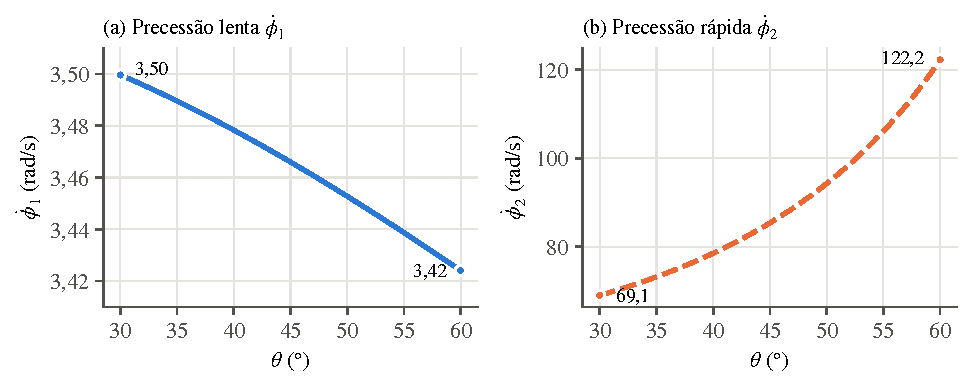
\includegraphics[width=\linewidth]{taxas_precessao.pdf}
\caption[Taxas de precessão permanente em função de $\theta$]{Taxas de precessão permanente em função de $\theta$: (a) solução lenta, praticamente constante; (b) solução rápida, fortemente crescente. As escalas verticais são distintas.}
\label{fig:taxas}
\end{figure}

As soluções reais existem somente se o discriminante da equação~\ref{eq:raizes} for não negativo. Essa exigência define o \textit{spin} mínimo da equação~\ref{eq:psimin}.
\begin{equation}
\psid \geq \psid_{\mathrm{min}} = \frac{2}{I}\sqrt{(I'-I)\cos\theta\;Wc}
\label{eq:psimin}
\end{equation}

Para $\theta=30^\circ$, a equação~\ref{eq:psimin} fornece $\psid_{\mathrm{min}}=80,8\un{rad/s}=771\un{rpm}$; para $\theta=60^\circ$, fornece $586\un{rpm}$. O valor de $1800\un{rpm}$ supera com folga esses limites, o que garante as duas soluções em toda a faixa estudada. Abaixo de $\psid_{\mathrm{min}}$, nenhuma precessão permanente é possível para a inclinação considerada.

\subsection{Item (b): condição para spin muito elevado}

Quando $\psid\gg\phid$, a equação~\ref{eq:compomega} fornece $\omega_z\approx\psid$. Além disso, o termo $I'\phid\cos\theta$ da equação~\ref{eq:condicao} torna-se desprezível em comparação com $I\psid$, e a condição de precessão permanente reduz-se à equação~\ref{eq:aprox}.
\begin{equation}
\phid_a \approx \frac{Wc}{I\psid} = \frac{mgc}{I\psid}
\label{eq:aprox}
\end{equation}

A equação~\ref{eq:aprox} é a resposta do item (b). Fisicamente, ela equivale a admitir $\vet{H}_O\approx I\psid\,\vet{k}$ na equação~\ref{eq:eulerM}: o momento do peso gira o vetor $\vet{H}_O$ à taxa $\phid$, o que nos leva à equação~\ref{eq:OmegaH_approx}:

\begin{equation}
Wc\seno\theta=\sum\vet{M}_O = \vOmega\times\vet{H}_O \approx \phid\,I\psid\seno\theta
\label{eq:OmegaH_approx}
\end{equation}

O fator $\seno\theta$ cancela-se e, por isso, a taxa aproximada independe da inclinação. Observa-se também que $\phid_a$ é inversamente proporcional ao \textit{spin}: quanto mais rápido gira o pião, mais lentamente precessa. Para os dados do problema, a equação~\ref{eq:aprox} fornece o valor da equação~\ref{eq:aproxnum}.
\begin{equation}
\phid_a = \frac{0,03924}{0,011781} = 3,331\un{rad/s} = 31,8\un{rpm}
\label{eq:aproxnum}
\end{equation}

Essa condição descreve apenas a raiz lenta $\phid_1$. Na raiz rápida, a razão $\phid_2/\psid$ varia de $0,37$ a $0,65$ na faixa estudada, de modo que a hipótese $\psid\gg\phid$ não é satisfeita.

\subsection{Item (c): erro da aproximação}

O erro relativo cometido ao aproximar $\phid_1$ por $\phid_a$ é definido pela equação~\ref{eq:erro}.
\begin{equation}
e = \frac{\phid_a-\phid_1}{\phid_1}\times100\%
\label{eq:erro}
\end{equation}

Para $\theta=30^\circ$, a equação~\ref{eq:erro} resulta no valor da equação~\ref{eq:erro30}. O sinal negativo indica que a aproximação subestima a taxa exata.
\begin{equation}
e = \frac{3,331-3,500}{3,500}\times100\% = -4,82\%
\label{eq:erro30}
\end{equation}

Pode-se obter uma expressão exata para o erro. Como $\phid_1$ é raiz da equação~\ref{eq:quad}, ela a satisfaz; isolando o termo linear em $\phid$, tem-se
\begin{equation}
b\,\phid_1 = Wc + a\,\phid_1^{\,2}.
\label{eq:erroinic}
\end{equation}
Dividindo ambos os membros por $b\,\phid_1$, resulta
\begin{equation*}
1 = \frac{Wc}{b\,\phid_1} + \frac{a\,\phid_1}{b}.
\end{equation*}
Pela equação~\ref{eq:aprox}, $\phid_a = Wc/b$, de modo que o primeiro termo do segundo membro é a razão $\phid_a/\phid_1$. Como, pela equação~\ref{eq:erro}, $e/100\% = \phid_a/\phid_1 - 1$, obtém-se a equação~\ref{eq:errofis}, que revela a origem do erro: ele é precisamente a parcela $a\,\phid_1^{\,2}$ desprezada na dedução da equação~\ref{eq:aprox}, na qual a equação~\ref{eq:quad} foi reduzida a $-b\,\phid + Wc = 0$.
\begin{equation}
\frac{e}{100\%} = -\frac{a\,\phid_1}{b} = -\frac{(I'-I)\cos\theta\;\phid_1}{I\psid}
\label{eq:errofis}
\end{equation}

A equação~\ref{eq:errofis} ainda depende de $\phid_1$. Para eliminá-lo, substitui-se a raiz lenta da equação~\ref{eq:raizes}:
\begin{equation*}
\frac{a\,\phid_1}{b}
= \frac{b-\sqrt{b^2-4aWc}}{2b}
= \frac{1-\sqrt{1-4aWc/b^2}}{2}.
\end{equation*}
Nessa forma, a razão $aWc/b^2$ aparece naturalmente. Definindo-a como o parâmetro adimensional $\eps=aWc/b^2$ e substituindo $a$ e $b$, o erro passa a ser dado em forma fechada pela equação~\ref{eq:errofechado}.
\begin{equation}
\frac{e}{100\%} = \frac{\sqrt{1-4\eps}-1}{2} \approx -\eps,
\qquad
\eps = \frac{(I'-I)\cos\theta\;Wc}{\left(I\psid\right)^2}
\label{eq:errofechado}
\end{equation}
A aproximação indicada na equação~\ref{eq:errofechado} decorre da expansão em série da raiz para $\eps \ll 1$,
\begin{equation}
\sqrt{1-4\eps} \approx 1 - 2\eps - 2\eps^2 - \cdots
\quad\Rightarrow\quad
\frac{e}{100\%} \approx -\eps - \eps^2 - \cdots,
\label{eq:erroserie}
\end{equation}
em que o termo de primeira ordem domina. Para $\theta = 30^\circ$, por exemplo, $\eps = 0,0459$ fornece $-4,82\%$ pela expressão exata e $-4,59\%$ apenas com $-\eps$.

A equação~\ref{eq:errofechado} mostra que o erro decresce com $\cos\theta$ e, para $\eps$ pequeno, é proporcional a $1/\psid^{\,2}$: dobrar o \textit{spin} reduz o erro a cerca de um quarto. A Tabela~\ref{tab:erro} resume os valores obtidos.

\begin{table}[H]
\centering
\caption{Erro da aproximação $\phid_a=3,331\un{rad/s}$ em relação à raiz lenta.}
\label{tab:erro}
\begin{tabular}{cccc}
\toprule
$\theta$ & $\phid_1$ (rad/s) & $\eps$ & $e$ (\%)\\
\midrule
$30^\circ$ & $3,500$ & $0,0459$ & $-4,82$\\
$35^\circ$ & $3,490$ & $0,0434$ & $-4,55$\\
$40^\circ$ & $3,478$ & $0,0406$ & $-4,24$\\
$45^\circ$ & $3,466$ & $0,0375$ & $-3,90$\\
$50^\circ$ & $3,453$ & $0,0341$ & $-3,53$\\
$55^\circ$ & $3,439$ & $0,0304$ & $-3,14$\\
$60^\circ$ & $3,424$ & $0,0265$ & $-2,72$\\
\bottomrule
\end{tabular}
\end{table}

A Figura~\ref{fig:erro} ilustra esses resultados. O painel (a) compara a taxa exata, levemente decrescente, com a aproximada, constante; o painel (b) mostra o módulo do erro, que diminui de $4,82\%$ para $2,72\%$ à medida que a inclinação aumenta.

\begin{figure}[H]
\centering
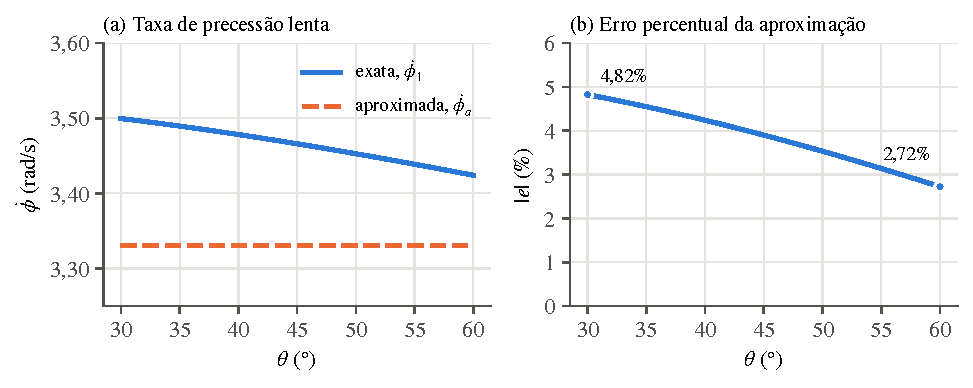
\includegraphics[width=\linewidth]{erro_aproximacao.pdf}
\caption[Comparação entre a solução exata e a aproximada]{Comparação entre a solução exata e a aproximada: (a) taxas de precessão lenta em função de $\theta$; (b) módulo do erro percentual da aproximação.}
\label{fig:erro}
\end{figure}

\subsection{Aprofundamento: influência do spin}

A Figura~\ref{fig:spin} amplia a análise para outros valores de \textit{spin}. No painel (a), em escala logarítmica e para $\theta=30^\circ$, as duas raízes nascem juntas em $\psid_{\mathrm{min}}$ (equação~\ref{eq:psimin}) e afastam-se à medida que o \textit{spin} aumenta: a raiz rápida cresce e a lenta decresce. A linha pontilhada marca o valor do problema. O painel (b), em escala bilogarítmica, confirma a tendência prevista pela equação~\ref{eq:errofechado}: o erro cai aproximadamente com $1/\psid^{\,2}$ e fica abaixo de $1\%$ a partir de cerca de $4000\un{rpm}$ para $\theta=30^\circ$.

\begin{figure}[H]
\centering
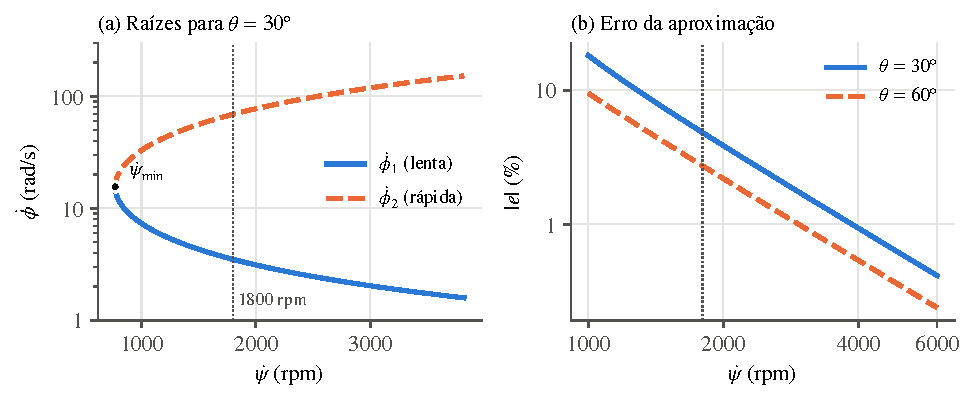
\includegraphics[width=\linewidth]{efeito_spin.pdf}
\caption[Influência do \textit{spin} nas raízes e no erro]{Influência do \textit{spin}: (a) raízes da equação de precessão para $\theta=30^\circ$; (b) erro da aproximação para $\theta=30^\circ$ e $\theta=60^\circ$. A linha pontilhada indica $1800\un{rpm}$.}
\label{fig:spin}
\end{figure}

\subsection{Aprofundamento: reações no apoio e energia}

Em precessão permanente, $G$ descreve uma circunferência horizontal de raio $c\seno\theta$ com velocidade angular $\phid$. A segunda lei de Newton fornece as reações em $O$ indicadas na Figura~\ref{fig:dcl}(b), cujas intensidades são dadas pela equação~\ref{eq:reacoes}.
\begin{equation}
N = W,
\qquad
R_h = mc\seno\theta\;\phid^{\,2}
\label{eq:reacoes}
\end{equation}

A energia mecânica do pião, com referência de energia potencial na altura de $O$, é expressa pela equação~\ref{eq:energia}.
\begin{equation}
E = \frac{1}{2}I'\phid^{\,2}\seno^2\theta + \frac{1}{2}I\omega_z^2 + Wc\cos\theta
\label{eq:energia}
\end{equation}

\subsection{Validação numérica}

Para verificar os resultados por um caminho independente, as equações do movimento foram integradas numericamente sem o uso da equação~\ref{eq:quad} nem dos ângulos de Euler. Empregou-se a equação de Euler do corpo rígido em eixos solidários ao pião (equação~\ref{eq:eulercorpo}), em conjunto com a cinemática de quatérnios (equação~\ref{eq:quat}), em que $\otimes$ denota o produto de quatérnios.
\begin{equation}
\vet{I}_O\cdot\dot{\vomega} + \vomega\times\left(\vet{I}_O\cdot\vomega\right) = \vet{M}_O
\label{eq:eulercorpo}
\end{equation}
\begin{equation}
\dot{\vet{q}} = \frac{1}{2}\,\vet{q}\otimes\left(0,\ \vomega\right)
\label{eq:quat}
\end{equation}

As equações~\ref{eq:eulercorpo} e~\ref{eq:quat} foram integradas com o método de Runge--Kutta de quarta ordem, com passo de $2\times10^{-5}\un{s}$ e duração de $1\un{s}$, em um programa escrito em Python. Os valores de $\theta$ e $\phi$ foram extraídos da orientação calculada do eixo de simetria.

% ------------------------------------------------------------- 3
\section{Resultados}

As respostas aos itens propostos são as seguintes.

\begin{itemize}
\item \textbf{Item (a):} para cada inclinação existem duas taxas de precessão permanente, listadas na Tabela~\ref{tab:raizes}. A lenta varia de $3,50\un{rad/s}$ ($33,4\un{rpm}$) em $\theta=30^\circ$ a $3,42\un{rad/s}$ ($32,7\un{rpm}$) em $\theta=60^\circ$; a rápida varia de $69,1\un{rad/s}$ ($659\un{rpm}$) a $122,2\un{rad/s}$ ($1167\un{rpm}$).
\item \textbf{Item (b):} para $\psid\gg\phid$, a condição é a da equação~\ref{eq:aprox}, que resulta em $\phid_a=3,33\un{rad/s}$ ($31,8\un{rpm}$), independentemente de $\theta$.
\item \textbf{Item (c):} a aproximação subestima a menor taxa de precessão, com erro de $4,82\%$ em $\theta=30^\circ$ e de $2,72\%$ em $\theta=60^\circ$ (Tabela~\ref{tab:erro}).
\end{itemize}

A Tabela~\ref{tab:fisica} compara as duas soluções com base nas equações~\ref{eq:compomega}, \ref{eq:reacoes} e~\ref{eq:energia}. Embora ambas sejam matematicamente válidas, elas diferem muito do ponto de vista físico.

\begin{table}[H]
\centering
\caption{Comparação física entre as precessões lenta e rápida.}
\label{tab:fisica}
\begin{tabular}{cccccc}
\toprule
$\theta$ & Solução & $\phid/\psid$ & $\omega_z$ (rad/s) & $E$ (J) & $R_h/W$\\
\midrule
$30^\circ$ & lenta & $0,019$ & $191,5$ & $1,181$ & $0,025$\\
           & rápida & $0,366$ & $248,3$ & $2,110$ & $9,72$\\
$45^\circ$ & lenta & $0,018$ & $191,0$ & $1,168$ & $0,035$\\
           & rápida & $0,453$ & $248,9$ & $2,419$ & $21,0$\\
$60^\circ$ & lenta & $0,018$ & $190,2$ & $1,151$ & $0,041$\\
           & rápida & $0,649$ & $249,6$ & $3,368$ & $52,8$\\
\bottomrule
\end{tabular}
\end{table}

Destaca-se a razão $R_h/W$. Na precessão lenta, a força horizontal no apoio é pequena, de até $4,1\%$ do peso: um coeficiente de atrito modesto já a sustentaria. Na precessão rápida, a força exigida atinge de $9,7$ a $53$ vezes o peso, algo que um pião simplesmente apoiado sobre um plano não poderia receber sem que a ponta deslizasse. Essa solução só é viável com o ponto $O$ efetivamente fixo, como admite o enunciado. Além disso, ela requer uma energia de $1,8$ a $2,9$ vezes maior. Fica assim explicado por que, na prática, observa-se apenas a precessão lenta.

A validação numérica confirmou os resultados analíticos. Iniciando a integração nas condições de cada raiz, para $\theta=30^\circ$, $45^\circ$ e $60^\circ$, a taxa de precessão calculada coincidiu com a da equação~\ref{eq:raizes} com desvio inferior a $10^{-8}\%$, o ângulo $\theta$ permaneceu constante com variação inferior a $10^{-8}$ graus e a energia foi conservada com variação relativa inferior a $10^{-11}$.

A Figura~\ref{fig:simulacao} mostra a simulação para $\theta_0=30^\circ$ e $\psid=1800\un{rpm}$, com o pião lançado exatamente com a taxa de precessão $\phid_1$. O ângulo $\theta$ permanece constante e $\phi$ cresce linearmente com o tempo, com inclinação igual a $\phid_1$, o que caracteriza a precessão permanente: o eixo do pião descreve um cone em torno da vertical, sem tombar.

\begin{figure}[H]
\centering
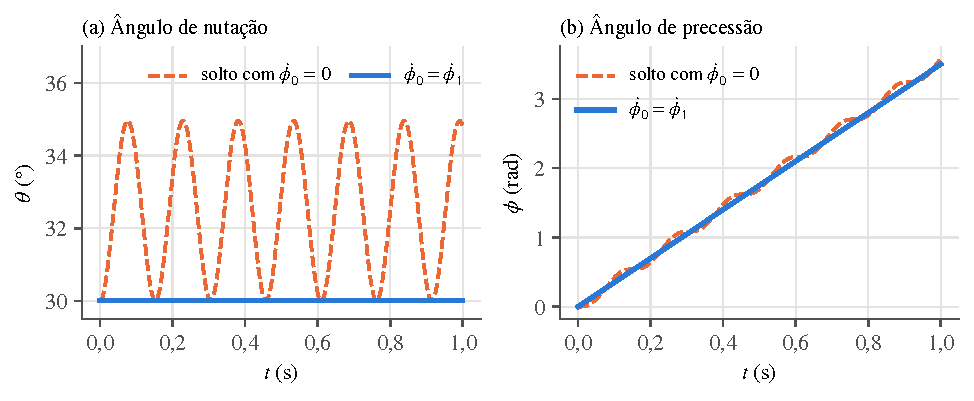
\includegraphics[width=0.6\linewidth]{simulacao.pdf}
\caption[Simulação numérica da precessão]{Simulação numérica do ângulo de precessão $\phi$ para $\theta_0=30^\circ$ e $\psid=1800\un{rpm}$, com taxa de precessão inicial igual à raiz lenta $\phid_1$.}
\label{fig:simulacao}
\end{figure}

% ------------------------------------------------------------- 4
\section{Conclusão}

O trabalho aplicou a dinâmica tridimensional do corpo rígido à precessão permanente de um pião. A partir dos ângulos de Euler e da segunda lei de Euler para o ponto fixo $O$, obteve-se uma equação de segundo grau para a taxa de precessão, cujas duas raízes foram calculadas para inclinações de $30^\circ$ a $60^\circ$. Verificou-se que o resultado não depende da massa do pião.

Para $\psid=1800\un{rpm}$, a taxa lenta permanece próxima de $3,5\un{rad/s}$ em toda a faixa, enquanto a rápida varia de $69$ a $122\un{rad/s}$. A condição simplificada $\phid_a\approx Wc/(I\psid)$ apresentou erro entre $2,72\%$ e $4,82\%$ em relação à raiz lenta, sempre por falta. Tal erro é aceitável para estimativas de engenharia e diminui rapidamente com o aumento do \textit{spin}, aproximadamente com o inverso de seu quadrado.

O aprofundamento mostrou que as duas soluções existem somente acima de um \textit{spin} mínimo. Mostrou também por que somente a precessão lenta é observada em um pião comum: a rápida exigiria forças horizontais muito superiores ao peso e uma energia consideravelmente maior. A integração numérica independente reproduziu as taxas de precessão previstas, com $\theta$ constante e energia conservada, o que confere confiança à solução.

O modelo tem limitações que convém registrar: o atrito é desprezado, de modo que o decaimento do \textit{spin} não é representado, e o ponto de apoio é considerado perfeitamente fixo. Em um pião real, a ponta tem dimensão finita e pode deslizar. Esses efeitos constituem extensões naturais do estudo.

% ------------------------------------------------------------- referências
\clearpage
\phantomsection
\addcontentsline{toc}{section}{Referências}
\begin{thebibliography}{9}
\bibitem{beer}
BEER, F. P.; JOHNSTON JR., E. R.; CORNWELL, P. J. \textit{Mecânica Vetorial para Engenheiros: Dinâmica}. 9. ed. Porto Alegre: AMGH, 2012.

\bibitem{goldstein}
GOLDSTEIN, H.; POOLE, C.; SAFKO, J. \textit{Classical Mechanics}. 3. ed. San Francisco: Addison-Wesley, 2002.
\end{thebibliography}

\end{document}